 \documentclass[a4paper,10pt]{article}
\include{amsymb}
\include{marvosym}

\usepackage[francais]{babel}
\usepackage[cyr]{aeguill}
\usepackage[applemac]{inputenc}
\usepackage{graphicx}
\usepackage{xspace}
\usepackage[a4paper]{geometry}
\usepackage{latexsym,amsmath,amssymb,textcomp}
\usepackage{moreverb}
\usepackage{listings}
\usepackage{multirow}
\usepackage{titling}
\usepackage{mathabx}

\usepackage{pdfpages}

\usepackage{hyperref}


\newlength{\indentationnota}
\newlength{\largeurlignenota}
\newlength{\paddingnota}
\newlength{\largeurnota}
\setlength{\paddingnota}{5pt}
\setlength{\largeurnota}{0.9cm}

\definecolor{pink}{rgb}{1,0.5,1}
\makeatletter

\newenvironment{pictonote}[1]{% on passe le nom du �chier en argument
\begin{list}{}{%
\setlength{\labelsep}{0pt}%
\setlength{\rightmargin}{15pt}%
\setlength{\paddingnota}{5pt}}
\item%
\setlength{\indentationnota}{%
\@totalleftmargin+\largeurnota+\paddingnota}%
\setlength{\largeurlignenota}{%
\linewidth-\largeurnota-\paddingnota}%
\parshape=3%
\indentationnota\largeurlignenota%
\indentationnota\largeurlignenota%
\@totalleftmargin\linewidth%
\raisebox{-\largeurnota+2.2ex}[0pt][0pt]{%
\makebox[0pt][r]{%
\includegraphics[width=\largeurnota]{#1}%
\hspace{\paddingnota}}}%
\ignorespaces}{%
\end{list}}

\makeatother

\newenvironment{attention}%
{\begin{pictonote}{/Users/benjamin/Documents/Education/LaTeX/danger}}%
{\end{pictonote}}

\newenvironment{unicorn}%
{\begin{pictonote}{/Users/benjamin/Documents/Education/LaTeX/angry_unicorn}}%
{\end{pictonote}}

\newcommand\unicornbox[1]{\colorbox{pink}{\color{white}{#1}}}

\newcommand\cf{\emph{c.f}}

\newcommand\signature{%
\begin{figure}[br]
	\begin{flushright}
	\begin{minipage}{8cm}
		\begin{center}
		\reflectbox{
\includegraphics[width=8cm]{/Users/benjamin/Documents/Education/LaTeX/unicorn}}\\
		\theauthor
		\end{center}
	\end{minipage}
	\end{flushright}
\end{figure}}

\newcommand\danger{\raisebox{-0.4ex}{\LARGE $\triangle$ \normalsize} \hspace{-4.1ex}! \hspace{1ex}}
\newcommand\PL{Programmation Logique\xspace}
\newcommand\pl{\bsc{Prolog}\xspace}


\title{TP2 : Codage d'un contour}
\author{Benjamin \bsc{Van Ryseghem} \\ Fran�ois \bsc{Lepan}}

\begin{document}
\maketitle

\section{Codage d'un contour}

\subsection{Comment sont cod�s les points du contour dans la variable cont?}
Les points du contour sont stock�s dans la variable sous forme d'une liste de nombres complexes. La valeur r�el correspondant � $x$ et la valeur imaginaire � $y$.

\subsection{En ne conservant qu'un point sur 4, puis un point sur 8, constituer deux autres contours approchant la forme circulaire et les afficher respectivement en bleu et en vert dans la m�me fen�tre}

Voici le code correspondant:

\begin{verbatim}
nom1 = "cercle-80.txt";
cont1 = rdfChargeFichierContour (nom1);

cont2 = cont1(1:4:$);
cont3 = cont1(1:8:$);
rdfAfficheContour(cont1, 2, "r");
rdfAfficheContour(cont2, 2, "g");
rdfAfficheContour(cont3, 2, "b");
\end{verbatim}

L'ex�cution du code pr�c�dent fournit la Fig.~\ref{fig:1_sur_4__1_sur_8}, sur laquelle apparaissent trois contours. Il y a d'abord le contour initial d'une forme circulaire repr�sent�e en rouge.

Il s'y trouve �galement le contour vert r�sultant du codage du contour original en ne conservant qu'un point sur quatre. 

Enfin, il y a le contour bleu repr�sentant le codage du contour original en ne gardant cette fois qu'un point sur huit.

\begin{figure}[ht]
	\begin{center}
		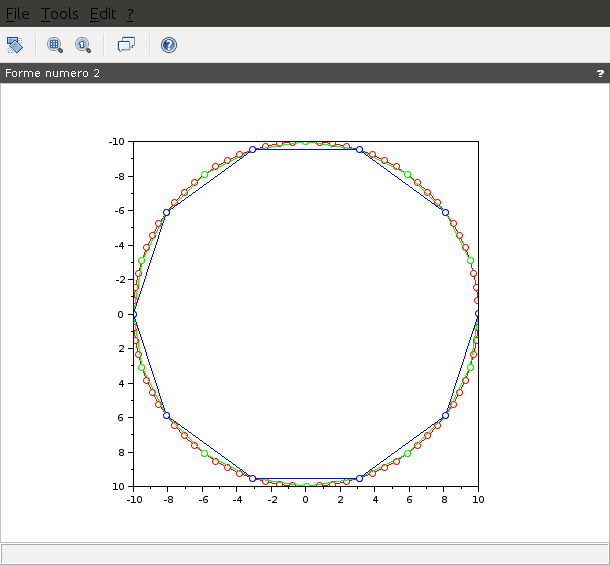
\includegraphics[width=13cm]{1_sur_4__1_sur_8.png}
	\end{center}
	\caption{rouge: contours initial \_\_ vert: 1 sur 4 \_\_ bleu: 1 sur 8}
	\label{fig:1_sur_4__1_sur_8}
\end{figure}


\section{Descripteur de Fourier}

\subsection{Pourquoi la fonction rdfDescFourier �limine t'elle parfois un point de la liste des points du contour?}
Pour plus de performance dans le calcule des descripteurs de Fourier.

\subsection{V�rifier que les descripteurs de Fourier permettent de reconstituer le contour initial}
Voici le code correspondant:
\begin{verbatim}
descFour = rdfDescFourier(cont);
rdfAfficheContour (rdfInverseDescFourier(descFour), 1, "k");
\end{verbatim}

\subsection{Quel est l'indice de tableau correspondant au descripteur Z0 ?}
C'est le premier �l�ment du tableau.

\subsection{Expliquer l'utilit� de la fonction rdfValeurDescFourier}
Cette fonction sert � afficher la valeur d'un point de la liste des descripteurs de Fourier 
 
 \subsection{� quoi correspond le descripteur de Fourier $Z_0$ d'une forme d�crite par son contour?}
 C'est le barycentre de la forme.
 
 On observe que si on change sa valeur on effectue une translation de l'image.
 
\begin{verbatim}
nom1 = "cercle-80.txt";
cont1 = rdfChargeFichierContour (nom1);
descFour = rdfDescFourier(cont1)
descFour1 = rdfDescFourier(cont1)
descFour1(1) = 5;

rdfAfficheContour(rdfInverseDescFourier(descFour), 2, "r");
rdfAfficheContour(rdfInverseDescFourier(descFour1), 2, "g");
\end{verbatim}

Le r�sultat de cette ex�cution fournit la Fig.~\ref{fig:chgmt_z0}, on y retrouve les deux contours du cercle. Le premier en rouge est la figure initial et le deuxi�me contour celui du m�me cercle mais translater de 5 unit�s.

\begin{figure}[ht]
	\begin{center}
		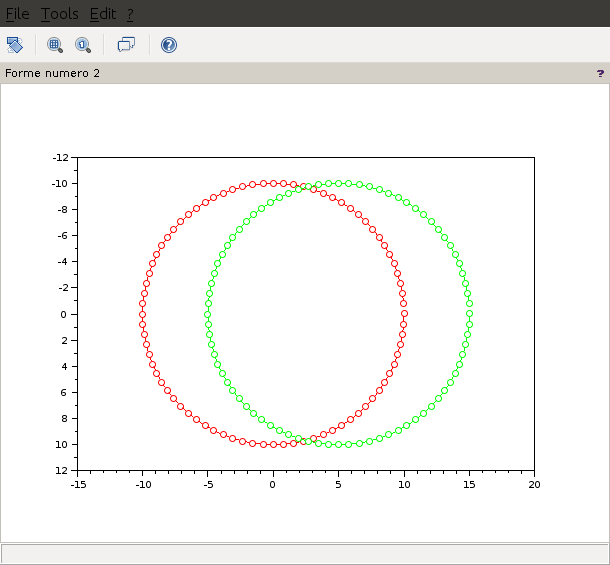
\includegraphics[width=12cm]{chgmt_z0.png}
	\end{center}
	\caption{rouge: contours initial \_\_ vert: 1 sur 4 \_\_ bleu: 1 sur 8}
	\label{fig:chgmt_z0}
\end{figure}

\section{Filtrage des descripteurs de Fourier}

Voici la fonction rdfAnnuleDescFourier:

\begin{verbatim}
function vector = rdfAnnuleDescFourier(desc,ratio)
    size = size(desc,1);
    
    if ratio == 1 then
        vector = desc
    else 
        if ratio == 0 then
            vector = zeros(1,size)
        else
            index = int(ratio*size)
            vector = [desc(1:index)' zeros(1,size-index) ]'
         end
    end
    
endfunction
\end{verbatim}


Lorsque nous r�duisons le ratio il se trouve qu'en effet la forme se simplifie (\emph{c.f.}~Fig.~\ref{fig:reduction_fourrier})

\begin{figure}[ht]
	\begin{center}
			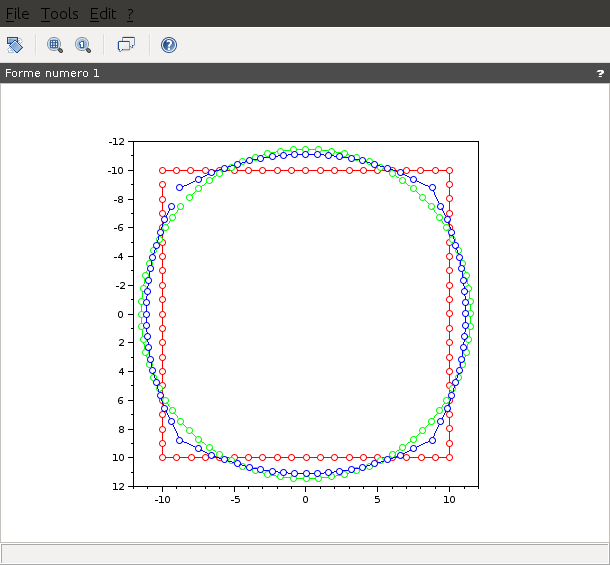
\includegraphics[width=10.7cm]{simplification_forme_desc_fourier.png}
	\end{center}
	\caption{Annulation des descripteurs de Fourrier: rouge: contour initial, bleu: ratio = 0.7, vert: ratio = 0.05}
	\label{fig:reduction_fourrier}
\end{figure}

\newpage

\section{R�duction d'une cha�ne de contour}

Voici le code que nous avons mis pour rdfAlgorithmeCorde:
\begin{verbatim}

    // Distances des autres points a la droite debut<->fin
    // le vecteur d, de meme taille que le vecteur
    // 'cont' doit contenir les distances

    // si c'est une droite verticale
    if real (debut) == real (fin)  then
        d = abs(real(cont) - real(debut))
    else	
        // on recupere le a et le b de ax + b
        a = (imag(fin) - imag(debut))/(real(fin) - real(debut))
        b = imag(fin) - a * real(fin)
        		
        // si c'est une droite horizontale
        if a == 0 then
            d = abs(imag(cont) - b)
        else
            d = abs(a*real(cont) - imag(cont) + b) ./ (sqrt(1+a^2))
        end
    end
\end{verbatim}



Et on observe bien que si on augmente \verb?dmax? on r�duit bien le nombre de point du contour (\emph{c.f.}~Fig.~\ref{fig:reduction_chaine_cont})


\begin{figure}[ht]
	\begin{center}
     		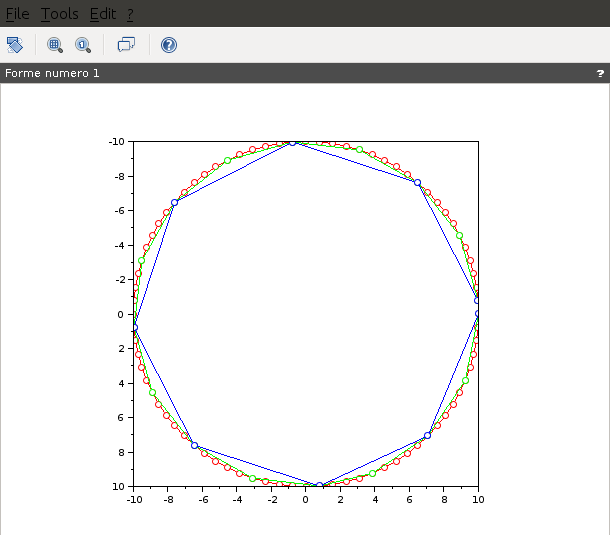
\includegraphics[width=9cm]{reduc_chaine_cont.png}
	\end{center}
	\caption{R�duction d'une chaine de contours. rouge: contours initial \_\_ vert:  Cordes avec dmax=0.5 \_\_ bleu  Cordes avec dmax=1}
	\label{fig:reduction_chaine_cont}
	
\end{figure}

\section{Comparaison des deux approches}

Apr�s avoir fait quelques tests nous nous sommes rendu compte que pour des formes connexes (triangles, carres, cercles) l'algorithme des cordes est mieux car beaucoup plus rapide que celui des descripteurs de Fourier. Cependant, dans les deux cas l'approximation est correcte (\emph{c.f.}~Fig.~\ref{fig:comp_fourier}).

\begin{figure}[ht]
	\begin{center}
		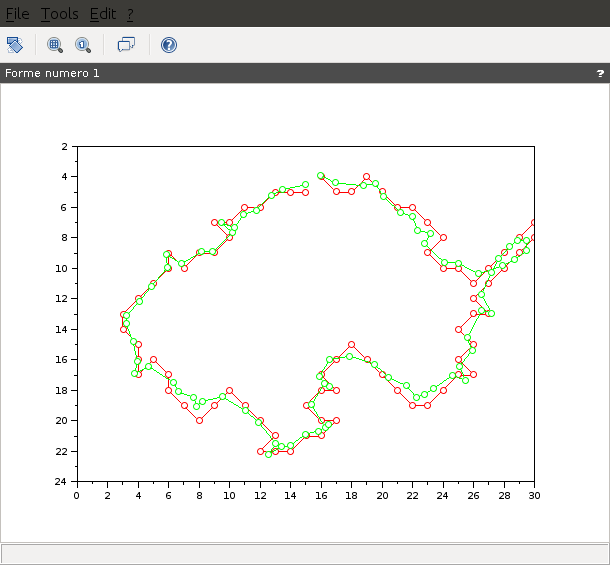
\includegraphics[width=12cm]{cmp_fourier_normale.png}
	\end{center}
	\caption{rouge: contours initial \_\_ vert: Fourier avec ratio=0.95 \_\_ bleu: Cordes avec dmax=1}
	\label{fig:comp_fourier}
\end{figure}

Mais pour ce qui est des formes non connexes (patato�de) l'algorithme de Fourier donne un meilleur aper�u de la forme d'origine. On observe sur la figure Fig.~\ref{fig:comp_fourier} que l'algorithme des cordes fait des segment qui sont moins repr�sentatif de la forme de base.

En conclusion nous dirons que l'algorithme des cordes est moins efficace pour faire de la reconnaissance de formes complexes comme un visage ou une patate (images r�elles) contrairement � l'algorithme de Fourier. Par contre il est beaucoup plus rapide pour des formes g�om�triques (images g�n�r�es) comme un triangle ou un carr�.
\end{document}